%TC:ignore
% ============================================================================
% TWO-STAGE RANDOMIZED TRIAL DESIGN FOR ANTIMICROBIALS: REVISED DRAFT
% Addresses reviewer feedback systematically
% ============================================================================

\documentclass[preprint,11pt]{elsarticle}

\usepackage{amsmath}
\usepackage{amssymb}
\usepackage{tikz}
\usepackage{lineno}
\usepackage{booktabs}
\usepackage{graphicx}
\usepackage{natbib}
\usepackage{multirow}
\usepackage{setspace}
\usetikzlibrary{shapes,arrows,arrows.meta,calc,positioning}

%TC:endignore

\begin{document}

\begin{frontmatter}

\title{Advantages of a Two-Stage Randomized Trial Design to Evaluate Antimicrobial Treatment Strategies: a Simulation Study}

\author[harvard]{Juan Gago\corref{cor1}}
\ead{juangago@hsph.harvard.edu}
\author[harvard,cwru,ccf]{Christopher Boyer}
\author[harvard]{Marc Lipsitch}

\cortext[cor1]{Corresponding author. 677 Huntington Avenue, Boston, MA, USA. Tel.: (917)459-7084.}

\address[harvard]{Department of Epidemiology, Harvard T.H. Chan School of Public Health, Boston, MA, USA}
\address[cwru]{Department of Medicine, Case Western Reserve School of Medicine, Cleveland, OH, USA}
\address[ccf]{Department of Quantitative Health Sciences, Cleveland Clinic, Cleveland, OH, USA}

\begin{abstract}
We present the simulation of a two-stage randomized trial study design evaluating antimicrobial treatment strategies using an agent-based model (ABM). The ABM simulates individuals in a hospital setting where bacterial transmission occurs. In the model, clusters follow a partial interference pattern, meaning there is interaction between patients (agents) within the cluster but no interaction between clusters. Agents exist in one of eleven states: not infected (X), infected with a drug-susceptible strain (S), or infected with a drug-resistant strain (R). Infected agents develop symptoms and enter treatment with one of two drugs: one targeting only susceptible strains (Drug A) or another targeting both susceptible and resistant strains (Drug B). Transmission, admission, discharge, symptom onset, treatment choice, and recovery are all modeled as stochastic events.

\textbf{Results:} The two-stage design successfully estimated direct effects of treatment choice (Drug~A recipients had 2.80--4.60 percentage points higher mortality than Drug~B recipients, attributable to non-concordant treatment of resistant infections) and indirect effects via altered population transmission dynamics. Under the high-use broad-spectrum strategy (50/50 allocation), there were fewer total deaths (603 vs.\ 888 under 90/10), driven by reduced resistant-strain mortality. However, the 50/50 strategy paradoxically led to a higher cumulative incidence of susceptible infections (9,625 vs.\ 7,599 under 90/10), because suppressing resistant strains released susceptible strains from competitive exclusion. This increase in susceptible infections---a spillover effect operating through altered transmission dynamics---would be undetectable in individually randomized trials but emerges naturally from the two-stage design by contrasting cluster-level strategies.

\textbf{Conclusion:} We found that antimicrobial prescribing policies interact with transmission dynamics in non-obvious ways through strain competition mechanisms. The two-stage randomized design is uniquely positioned to capture these indirect effects and spillover phenomena that conventional individually randomized trials cannot measure.

\end{abstract}

\begin{keyword}
causal inference \sep interference \sep drug resistance \sep antibiotics \sep agent-based models
\end{keyword}

\end{frontmatter}

\clearpage
\doublespacing

\section{Introduction}\label{sec:intro}

Antimicrobial resistance (AMR) threatens to undermine many of the gains of modern medicine by reducing the effectiveness of treatments for common infections. The challenge for clinicians and policymakers is to identify antimicrobial strategies that achieve two goals simultaneously: treating infections effectively in the individual patient and limiting the emergence and spread of resistance in the population.

Most of the available evidence on antimicrobial therapies comes from individually randomized controlled trials. These trials are designed to estimate the causal effect of treatment assignment on outcomes in the treated patient. However, because they randomize individuals in isolation, they provide little information about spillover effects---that is, how the treatment of one patient may affect the outcomes of others. Ignoring these indirect effects is problematic because antimicrobial use in one individual can alter the risk faced by others through transmission of both susceptible and resistant organisms.

Two-stage randomized (2SR) designs provide a framework for simultaneously estimating direct and indirect effects. In these designs, clusters (e.g., hospital wards) are first randomized to different levels of treatment coverage, and then individuals within clusters are randomized to treatment strategies consistent with the cluster assignment. Such designs have been applied in the evaluation of vaccines and HIV prevention interventions, where indirect effects are expected to be substantial \citep{buchanan_disseminated_2021}. Recent methodological work has formalized how 2SR trials can be understood within the target trial framework and emulated using simulation models \citep{murray_emulating_2021}. To our knowledge, no applications of this approach have yet been developed specifically for antimicrobial treatment strategies, despite the fact that indirect effects are central to the dynamics of AMR \citep{gago_how_2025}.

Other approaches have attempted to address the challenge of measuring AMR at the population level. Observational studies and mechanistic transmission models suggest that antimicrobial use influences resistance prevalence at the population level \citep{pham_characterizing_2025, olesen_role_2020, lipsitch_epidemiology_2000}, but these designs face well-known threats to causal identification. A few cluster-randomized antimicrobial trials exist---for example, Van Duijn et al.\ (2018) \citep{duijn_effects_2018} and the mass azithromycin trial in Niger \citep{arzika_spillover_2025}--- although it is not common to find attempts to estimate both direct and spillover effects when evaluating antimicrobial treatment strategies. Agent-based models (ABMs) have also been used to explore related questions, such as the evaluation of carbapenem-resistant Enterobacterales decolonization strategies \citep{toth_economic_2021}, but they have not yet been explicitly structured to emulate 2SR designs for antimicrobials.

In this paper, we extend the 2SR framework to antimicrobial strategies by implementing it in an ABM. Specifically, we define clusters as hospital wards and randomize both cluster-level coverage (the proportion of patients treated with broad-spectrum Drug B) and individual-level treatment assignment (which specific drug a patient receives). By doing so, our simulation generates causal contrasts that are unbiased by design under the model assumptions. The ABM serves as the data-generating mechanism from which the target 2SR trial is emulated, with clusters as the unit of first-stage randomization and individuals as the unit of second-stage randomization. This allows us to quantify direct, indirect, and overall effects of antimicrobial prescribing policies under controlled, simulated conditions.

Our work provides the first formal evaluation of a two-stage randomized design for antimicrobial treatment strategies. This approach establishes a framework that can inform both the design of future randomized trials and the emulation of such trials with observational data. It also offers insights into how stewardship interventions may affect resistance dynamics at both the patient and population level.

\section{Methods}

\subsection{Model Setup Description}\label{MODEL}

We developed a discrete-time, stochastic agent-based model (ABM) to simulate a two-stage randomized trial of antimicrobial treatment strategies in a hospital setting. Each agent represents an individual patient followed over 350 timesteps within a simulated ward structure. We used R software version 4.4.1 and the ABM package (version 0.4.3) for simulations.

Each agent occupies one of the following mutually exclusive health states:
\[
X,\quad S,\quad R,\quad US,\quad TS_A,\quad TS_B,\quad UR,\quad TR_A,\quad TR_B,\quad Z,\quad D
\]
where:
\begin{itemize}
  \item $X$: susceptible (uninfected),
  \item $S$: infected with a drug-susceptible strain,
  \item $R$: infected with a drug-resistant strain,
  \item $US$, $UR$: untreated susceptible or resistant infections,
  \item $TS_A$, $TS_B$: treated susceptible infections with Drug A or B, respectively,
  \item $TR_A$, $TR_B$: treated resistant infections with Drug A or B, respectively,
  \item $Z$: discharged alive,
  \item $D$: deceased.
\end{itemize}

The model dynamics are defined by the following stochastic processes:

\subsubsection{Admission and Discharge}
\begin{itemize}
  \item Admissions follow a Poisson process at rate $\lambda = 10$.
  \item New admissions enter state $X$ (uninfected) with probability $m = 0.75$, or state $S$ (susceptible infection) with probability $1 - m$. No new admissions arrive with resistant infections; all resistance in the model arises from within-ward transmission.
  \item Discharge alive ($Z$) and death ($D$) transitions apply only to symptomatic or treated agents (states $TS_A$, $TS_B$, $US$, $TR_A$, $TR_B$, $UR$). Discharge occurs at rate $\mu = 0.095$; death occurs at rate $\delta = 0.025$ multiplied by a state-specific factor (see Section~\ref{sec:mortality}).
\end{itemize}

\subsubsection{Transmission}
Homogeneous mixing within wards (justified by the assumption of adequate contact rates and proximity within wards) leads to:
\[
  X + S \xrightarrow{\beta} S + S, \qquad
  X + R \xrightarrow{\beta(1 - c)} R + R,
\]
where $\beta = 0.4$ is the transmission rate and $c = 0.02$ is the fitness cost of resistance (reducing transmissibility of resistant strains).

\subsubsection{Symptom Onset and Treatment}
\begin{itemize}
  \item Symptom onset occurs at rate $\sigma = 1$. (This rate assumes rapid symptom development, effectively collapsing the latent period.)
  \item Given symptoms, patients enter treatment with probability $\rho = 0.9$:
    \begin{itemize}
      \item Drug A (covers susceptible strains) with probability $\pi$ (cluster-specific: 0.9 or 0.5),
      \item Drug B (covers both susceptible and resistant strains) with probability $1 - \pi$.
    \end{itemize}
  \item Untreated symptomatic patients remain in $US$ or $UR$.
\end{itemize}

\subsubsection{Recovery}
Recovery transitions are set as follows:
\[
  TS_A,\, TS_B \xrightarrow{\gamma_S + \tau} X, \quad
  US \xrightarrow{\gamma_S} X,
\]
\[
  TR_A \xrightarrow{\gamma_R} X, \quad
  TR_B \xrightarrow{\gamma_R + \tau} X, \quad
  UR \xrightarrow{\gamma_R} X,
\]
with $\gamma_S = \gamma_R = 0.20$ and treatment effect $\tau = 0.7$. The treatment effect accelerates recovery (and reduces the infectious period) for patients receiving the appropriate drug. This applies to $TS_A$ and $TS_B$ for susceptible infections (both drugs cover $S$), but only to $TR_B$ for resistant infections (only Drug B covers $R$).

\subsection{Parameter Values and Justifications}

\begin{table}[htbp]
\centering
\caption{Model parameters: definitions, values, and justifications.}
\label{tab:parameters}
\begin{tabular}{llll}
\toprule
\textbf{Parameter} & \textbf{Symbol} & \textbf{Value} & \textbf{Justification} \\
\midrule
Admission rate (per timestep) & $\lambda$ & 10 & Maintains ward at $\approx 1000$ agents \\
Probability X admission & $m$ & 0.75 & Reflects baseline prevalence of uninfected \\
Initial susceptible infected & $S_0$ & 50 & Seeds infection pressure \\
Initial resistant infected & $R_0$ & 50 & Comparable resistance burden \\
Transmission rate & $\beta$ & 0.4 & Within-ward contact rate \\
Fitness cost of resistance & $c$ & 0.02 & Reduced transmissibility of R strains \\
Recovery rate (S and R) & $\gamma_S, \gamma_R$ & 0.20 & Mean duration $1/\gamma = 5$ timesteps \\
Treatment effect & $\tau$ & 0.7 & Reduces mean infectious period by 78\% \\
Symptom onset rate & $\sigma$ & 1.0 & Rapid onset (collapsing latent period) \\
Prob. treatment given symptoms & $\rho$ & 0.9 & High treatment uptake \\
Discharge rate & $\mu$ & 0.095 & Balances admission rate for stability \\
Baseline death rate & $\delta$ & 0.025 & 2.5\% baseline mortality \\
Prob.\ Drug A (high-A strategy, $\alpha_1$) & $\pi$ & 0.90 & 90\% Drug A, 10\% Drug B \\
Prob.\ Drug A (balanced strategy, $\alpha_0$) & $\pi$ & 0.50 & 50\% Drug A, 50\% Drug B \\
\bottomrule
\end{tabular}
\\
\footnotesize
\textit{Note:} Sensitivity analyses were performed on $\tau$, $\beta$, $\delta$, and number of clusters.
\end{table}

\subsection{Simulation Procedure}

\begin{itemize}
  \item We initialize 1,000 agents ($n = 1000$), where 50 are in state $S$ and 50 are in state $R$; all remaining agents are uninfected ($X$).
  \item Event rates (admissions, transmissions, symptom onset, treatment, recovery, discharge, death) occur over $T = 350$ timesteps.
  \item We simulate $n_{\text{clus}} = 6$ clusters with 3 clusters assigned to $\pi = 0.9$ (90/10 strategy) and 3 assigned to $\pi = 0.5$ (50/50 strategy).
  \item We replicate each cluster scenario $s = 10$ times to capture stochastic variability.
  \item Ward occupancy remains approximately stable over the simulation period, as admission rates balance discharge and death rates.
\end{itemize}

\subsection{Causal Inference Assumptions}

We define causal effects within a potential outcomes framework under the assumption of \textit{partial interference} \citep{hudgens_toward_2008, sobel_what_2006}. Let $\mathbf{z}_i = (z_{i1}, \ldots, z_{in_i})$ denote the vector of treatment assignments for all $n_i$ individuals in cluster $i$, where $z_{ij} \in \{A, B\}$ denotes the drug assigned to individual $j$. The potential outcome for individual $j$ in cluster $i$ is $Y_{ij}(\mathbf{z}_i)$, which depends on the entire treatment vector of their cluster.

We make two key assumptions. First, \textit{partial interference}: an individual's outcome may depend on treatments assigned to others in their cluster, but not on treatments in other clusters. That is,
\begin{equation}
Y_{ij}(\mathbf{z}_1, \ldots, \mathbf{z}_K) = Y_{ij}(\mathbf{z}_i).
\end{equation}
This assumption is justified by the homogeneous within-cluster mixing and the absence of cross-cluster transmission in our model.

Second, \textit{stratified interference} \citep{hudgens_toward_2008}: the potential outcome $Y_{ij}(\mathbf{z}_i)$ depends on $\mathbf{z}_i$ only through (a) the individual's own treatment $z_{ij}$ and (b) the proportion of cluster members assigned to each drug (i.e., the allocation strategy $\alpha_i$). Under this assumption, we can write
\begin{equation}
Y_{ij}(\mathbf{z}_i) = Y_{ij}(\mathbf{z}_i') \quad \text{for all } \mathbf{z}_i, \mathbf{z}_i' \text{ such that } z_{ij} = z_{ij}' \text{ and } \alpha(\mathbf{z}_i) = \alpha(\mathbf{z}_i'),
\end{equation}
where $\alpha(\mathbf{z}_i)$ denotes the proportion of Drug A assignments in cluster $i$.

These two assumptions relax the standard Stable Unit Treatment Value Assumption (SUTVA), which would require no interference between agents \citep{hudgens_toward_2008}. The stratified interference assumption enables us to define \textit{individual average potential outcomes} $\bar{Y}_{ij}(a, \alpha)$: the expected outcome for individual $j$ in cluster $i$ when assigned treatment $a$ under allocation strategy $\alpha$, averaging over all compatible treatment vectors for other cluster members. All causal estimands below are defined as contrasts of population averages of $\bar{Y}_{ij}(a, \alpha)$.

Because we implemented a two-stage randomized design---clusters randomized to allocation strategy $\alpha_i \in \{\alpha_0, \alpha_1\}$ (corresponding to 50/50 and 90/10 strategies, respectively), then individuals randomized to $z_{ij} \in \{A, B\}$ within clusters---we preserve \textit{exchangeability by design} at both levels. The assumptions of \textit{consistency} (the observed outcome under assigned treatment equals the potential outcome under that treatment) and \textit{positivity} (non-zero probability of treatment assignment at each level) are built-in properties of the simulation design. Full adherence to assigned treatment probabilities and fixed cluster sizes mean that inverse probability weighting is not required for the simulation analysis. However, when emulating this design with observational data, confounding adjustment at both the cluster and individual levels (e.g., via inverse probability weighting or g-computation) would be essential \citep{tchetgen_tchetgen_causal_2012}.

\subsection{Mortality Rates by Stratum}\label{sec:mortality}

The outcome in our simulation is all-cause mortality. We set a baseline death rate of $\delta = 0.025$. Under our model, the per-state mortality hazards are:
\begin{itemize}
  \item Treated susceptible ($TS_A$, $TS_B$): $1 \times \delta = 0.025$
  \item Untreated symptomatic susceptible ($US$): $1.5 \times \delta = 0.0375$
  \item Treated resistant, concordant ($TR_B$): $1 \times \delta = 0.025$
  \item Treated resistant, non-concordant ($TR_A$): $2 \times \delta = 0.05$
  \item Untreated symptomatic resistant ($UR$): $3 \times \delta = 0.075$
\end{itemize}

These rates reflect the assumption that untreated infections carry higher mortality, that resistant infections treated with a non-concordant drug (Drug~A, which does not cover $R$) have elevated mortality, and that concordant treatment (Drug~B for $R$ infections, or either drug for $S$ infections) returns mortality to the baseline rate. Note that discharge from states $X$, $S$, and $R$ (pre-symptomatic or uninfected) does not occur in our model; only symptomatic or treated agents are subject to discharge and death transitions. Pre-symptomatic agents transition rapidly to symptomatic states given $\sigma = 1$.

\subsection{Outcome Measures and Causal Estimands}

The primary outcome of interest is all-cause mortality. Let $\bar{Y}(a, \alpha)$ denote the population average of the individual average potential outcomes under treatment $a$ and allocation strategy $\alpha$, and let $\bar{Y}(\alpha)$ denote the marginal population average under strategy $\alpha$, averaging over individual treatment assignment. We define the following causal estimands, following \citet{hudgens_toward_2008}:

\begin{align}
\mathrm{DE}(\alpha_0) &= \bar{Y}(A,\, \alpha_0) \;-\; \bar{Y}(B,\, \alpha_0), \label{eq:de0}\\[4pt]
\mathrm{DE}(\alpha_1) &= \bar{Y}(A,\, \alpha_1) \;-\; \bar{Y}(B,\, \alpha_1), \label{eq:de1}\\[4pt]
\mathrm{IE}(A) &= \bar{Y}(A,\, \alpha_1) \;-\; \bar{Y}(A,\, \alpha_0), \label{eq:iea}\\[4pt]
\mathrm{IE}(B) &= \bar{Y}(B,\, \alpha_1) \;-\; \bar{Y}(B,\, \alpha_0), \label{eq:ieb}\\[4pt]
\mathrm{TE} &= \bar{Y}(A,\, \alpha_1) \;-\; \bar{Y}(B,\, \alpha_0), \label{eq:te}\\[4pt]
\mathrm{OE} &= \bar{Y}(\alpha_0) \;-\; \bar{Y}(\alpha_1), \label{eq:oe}
\end{align}

where $\alpha_0$ denotes the 50/50 strategy (50\% Drug~A, 50\% Drug~B) and $\alpha_1$ denotes the 90/10 strategy (90\% Drug~A, 10\% Drug~B).

\begin{itemize}
  \item $\mathrm{DE}(\alpha)$: The \textit{direct effect} of Drug~A vs.\ Drug~B within a fixed allocation strategy. This isolates the effect of one's own treatment, holding the cluster environment constant.
  \item $\mathrm{IE}(a)$: The \textit{indirect (spillover) effect} of the allocation strategy (90/10 vs.\ 50/50) among recipients of a given drug. This captures how the treatment environment affects outcomes through altered transmission, holding one's own treatment fixed.
  \item $\mathrm{TE}$: The \textit{total effect}, which combines both the direct and indirect effects. Following \citet{hudgens_toward_2008}, the TE decomposes as either $\mathrm{TE} = \mathrm{DE}(\alpha_1) + \mathrm{IE}(B)$ or equivalently $\mathrm{TE} = \mathrm{IE}(A) + \mathrm{DE}(\alpha_0)$. It compares Drug~A recipients under 90/10 to Drug~B recipients under 50/50.
  \item $\mathrm{OE}$: The \textit{overall effect}, marginalizing over individual treatment assignment. This is the most policy-relevant estimand, representing the expected population-level impact of shifting the entire prescribing strategy from 50/50 to 90/10.
\end{itemize}

\textit{Note on sign convention:} All estimands are defined such that positive values indicate higher mortality (i.e., worse outcomes) in the first term relative to the second. The OE is defined as $\alpha_0$ (50/50) minus $\alpha_1$ (90/10), so a negative OE indicates that the 50/50 strategy reduces mortality.

\subsubsection{Inference and Simulation Intervals}

Point estimates of all causal effects were computed by averaging the outcome across simulation replicates. Ninety-five percent simulation intervals (SI) were computed as the empirical 2.5th and 97.5th percentiles of the distribution of point estimates across 10 replicates per cluster-strategy combination. Simulation intervals reflect Monte Carlo variability in the model but do not quantify uncertainty due to model misspecification or parameter uncertainty.

\subsection{Sensitivity Analyses}\label{sec:sa_methods}

We conducted a series of one-way sensitivity analyses to assess the robustness of our findings to key model assumptions. Four dimensions were varied independently, holding all other parameters at their base-case values:

\begin{enumerate}
  \item \textit{Mortality structure (uniform hazards):} We re-ran the simulation with uniform mortality hazards across all infection-treatment combinations, setting $\delta = 0.025$ constant across all states. This eliminated differential mortality severity and allowed assessment of whether spillover effects persist independently of outcome severity differences.

  \item \textit{Treatment effect magnitude:} We varied $\tau \in \{0.3, 0.7, 1.0\}$ to test whether the magnitude of the treatment-induced recovery acceleration affects the direction or magnitude of indirect and overall effects.

  \item \textit{Transmission rate:} We varied $\beta \in \{0.2, 0.4, 0.6\}$ to assess whether spillover effects depend on the intensity of within-ward transmission.

  \item \textit{Cluster configuration:} We tested 3 clusters per arm (base case, 10 replicates each) against 6 clusters per arm (5 replicates each) to evaluate stability of effect estimates with increasing numbers of clusters.
\end{enumerate}

\subsection{Compartment Diagram}

\begin{figure}[ht!]
  \centering
  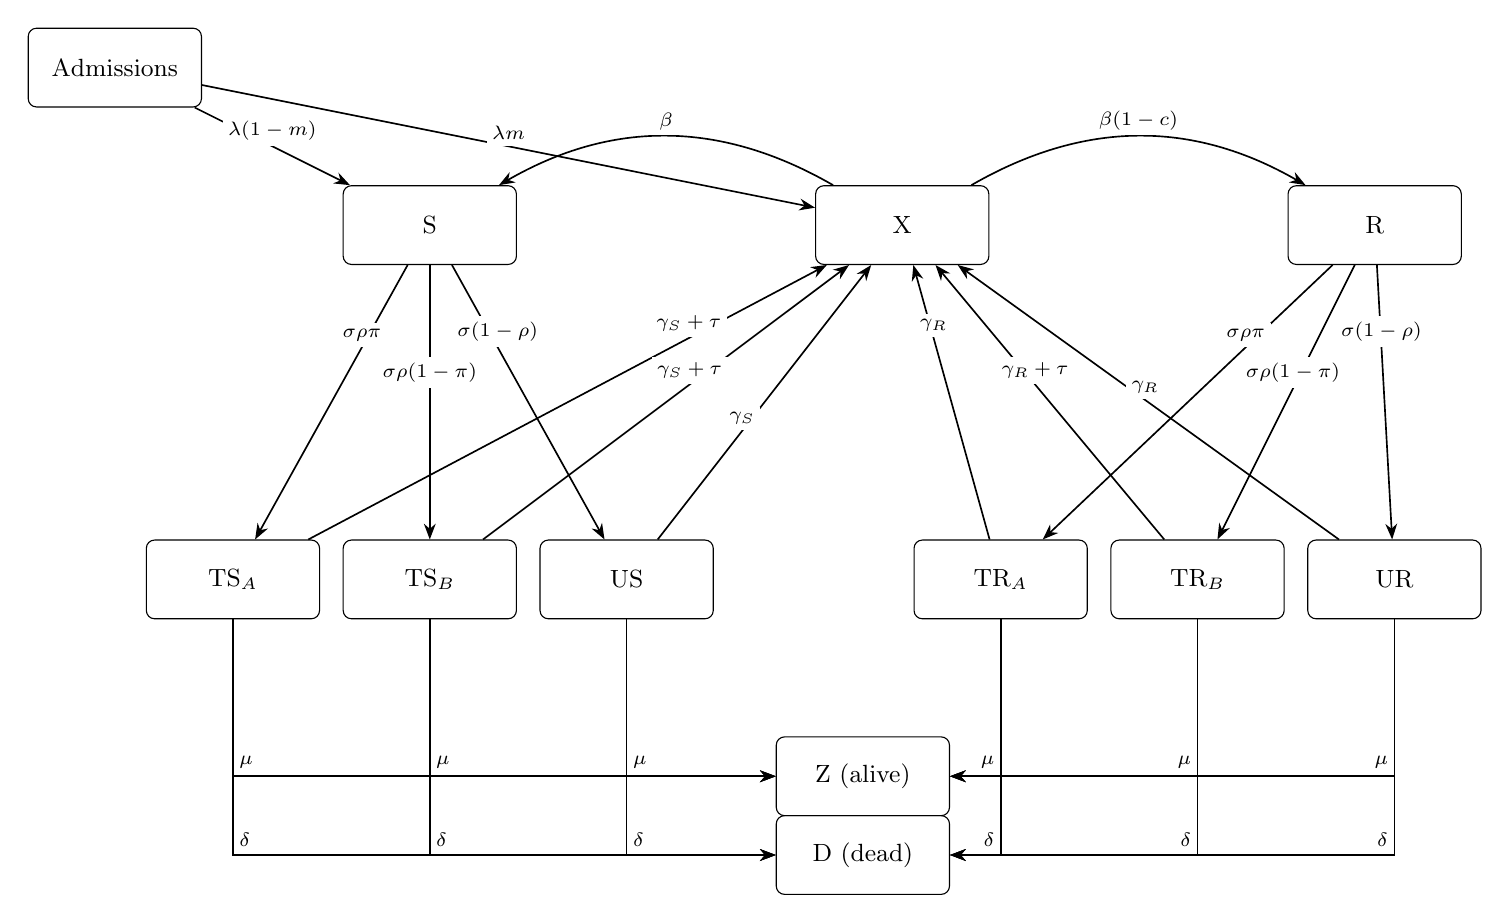
\begin{tikzpicture}[
    >=Stealth,
    box/.style  = {draw, rounded corners=3pt,
                   minimum width=22mm, minimum height=10mm,
                   align=center, font=\small},
    trans/.style = {semithick,->},
    lbl/.style   = {font=\scriptsize, midway, inner sep=2pt, fill=white}
  ]
  \draw[transform canvas={xshift = -10cm}] ;

  %–––– grid coordinates ––––
  \coordinate (origin) at (0,0);

  % second (colonisation) tier
  \node[box] (S) at ($(origin)+( 0, 0)$) {S};
  \node[box] (X) at ($(origin)+( 6, 0)$) {X};
  \node[box] (R) at ($(origin)+(12, 0)$) {R};

  % third (symptom/treatment) tier –– left block
  \node[box] (TSA) at ($(S)+( -2.5,-4.5)$) {$\mathrm{TS}_A$};
  \node[box] (TSB) at ($(S)+(  0,-4.5)$) {$\mathrm{TS}_B$};
  \node[box] (US)  at ($(S)+( 2.5,-4.5)$) {US};

  % third tier –– right block
  \node[box] (TRA)  at ($(R)+( -4.75,-4.5)$) {$\mathrm{TR}_A$};
  \node[box] (TRB) at ($(R)+(  -2.25,-4.5)$) {$\mathrm{TR}_B$};
  \node[box] (UR)  at ($(R)+( 0.25,-4.5)$) {UR};

  % admission box (top left)
  \node[box] (ADM) at ($(S)+(-4, 2)$) {Admissions};

  % discharge/death sink (bottom centre)
  \node[box] (Z)  at ($(X)+( -0.5,-7)$) {Z (alive)};
  \node[box] (D)  at ($(X)+(  -0.5,-8)$) {D (dead)};

  %–––– admission ––––
  \draw[trans] (ADM) -- (S)   node[lbl,above] {$\lambda(1-m)$};
  \draw[trans] (ADM) -- (X)                node[lbl,above]{$\lambda m$};

  %–––– symptom onset / treatment choice ––––
  % Symptom onset & treatment for susceptible
  \draw[trans] (S) -- (TSA) node[lbl,pos=0.3,above] {$\sigma\rho \pi$};
  \draw[trans] (S) -- (TSB) node[lbl,pos=0.45,above] {$\sigma\rho(1-\pi)$};
  \draw[trans] (S) -- (US)  node[lbl,pos=0.3,above] {$\sigma(1-\rho)$};

  % Symptom onset & treatment for resistant
  \draw[trans] (R) -- (TRA) node[lbl,pos=0.3,above] {$\sigma\rho \pi$};
  \draw[trans] (R) -- (TRB) node[lbl,pos=0.45,above] {$\sigma\rho(1-\pi)$};
  \draw[trans] (R) -- (UR)  node[lbl,pos=0.3,above] {$\sigma(1-\rho)$};

  %–––– recovery arrows ––––
  \draw[trans]   (TSA) -- ($(TSA)!0.55!(X)$) node[lbl,pos=1.3,above] {$\gamma_S+\tau$} -- (X);
  \draw[trans]   (TSB) -- ($(TSB)!0.55!(X)$) node[lbl,pos=1,above] {$\gamma_S+\tau$} -- (X);
  \draw[trans]   (US)  -- ($(US)!0.55!(X)$)  node[lbl,pos=0.7,above] {$\gamma_S$}     -- (X);

  \draw[trans]   (TRA) -- ($(TRA)!0.55!(X)$) node[lbl,pos=1.3,above] {$\gamma_R$}     -- (X);
  \draw[trans]   (TRB) -- ($(TRB)!0.55!(X)$) node[lbl,pos=1,above] {$\gamma_R+\tau$}-- (X);
  \draw[trans]   (UR)  -- ($(UR)!0.55!(X)$)  node[lbl,pos=0.9,above] {$\gamma_R$}     -- (X);

  %–––– transmission ––––
  \draw[trans]   (X) to[out=30,in=150,looseness=1]
      node[lbl,above] {$\beta(1-c)$}   (R);

  \draw[trans]    (X) to[out=150,in=30,looseness=1]
      node[lbl,above] {$\beta$}   (S);

  % discharge & death arrows
  \foreach \n in {TSA,TSB,US} {
  \draw[trans] (\n.south) -- ++(0,-7mm) node[lbl,pos=2.6, right]{$\mu$} |- (Z.west);
  \draw[trans] (\n.south) -- ++(0,-7mm) node[lbl, pos= 4, right]{$\delta$} |- (D.west);
  }

  \foreach \n in {TRA,TRB,UR} {
  \draw[trans] (\n.south) -- ++(0,-7mm) node[lbl,pos=2.6, left]{$\mu$} |- (Z.east);
  \draw[trans] (\n.south) -- ++(0,-7mm) node[lbl, pos= 4, left]{$\delta$} |- (D.east);
  }

  \end{tikzpicture}
  \caption{State-transition diagram for the hospital transmission ABM. Arrow labels give transition rates or probabilities. Identical discharge/death flows ($\mu$) are routed to a single sink for clarity. This ABM is replicated for each cluster, with all transition rates preserved except for transitions from $S$ and $R$ to treatment compartments, which depend on the cluster-level allocation strategy.}
  \label{fig:abm-diagram}
\end{figure}

\section{Results}

The simulation comprised 6 hospital wards (clusters), with 3 randomized to the 90/10 allocation strategy (90\% Drug A, 10\% Drug B) and 3 to the 50/50 strategy (50\% Drug A, 50\% Drug B). Each cluster was simulated 10 times to capture stochastic variability, yielding 60 total simulation runs. Each ward was initialized with 1,000 agents, with mean admissions of 10 per timestep and discharge and death rates approximately balancing the admission flow. Under the 50/50 strategy, resistant strains were suppressed while susceptible infections dominated; under the 90/10 strategy, resistant strains persisted at higher prevalence.

\subsection{Formal Causal Estimands}

Table~\ref{tab:estimands} presents the primary causal effect estimates. The direct effect of Drug~A versus Drug~B was positive under both allocation strategies (DE($\alpha_0$) = $+2.80$~percentage points; DE($\alpha_1$) = $+4.60$~percentage points), indicating higher mortality among Drug~A recipients. This is expected: Drug~A does not cover resistant infections, so patients with resistant infections treated with Drug~A face the elevated TR$_A$ mortality rate ($2\delta = 0.05$), while Drug~B covers both strain types. The direct effect is larger under the 90/10 strategy, where greater Drug~A use means a larger fraction of resistant-infected patients receive non-concordant therapy.

For Drug~B recipients, the indirect effect was approximately null (IE(B) = $-0.05$~percentage points; 95\% SI [$-0.90$, $+0.46$]), suggesting minimal spillover on B-treated patients' mortality. For Drug~A recipients, the indirect effect was positive and larger (IE(A) = $+1.75$~percentage points; 95\% SI [$+0.72$, $+3.49$]), reflecting that when Drug~A use is high (90/10 strategy), A-treated patients face a ward environment with substantially higher resistant-strain prevalence; since Drug~A does not cover resistant infections, this shifts the case mix toward resistant infections treated with a non-concordant drug, raising mortality. These patterns are visible in Figure~\ref{fig:cumulative_deaths}, where panel~(A) shows the 90/10 strategy producing substantially more resistant-strain deaths, while panel~(B) reveals that even susceptible-strain deaths---where both drugs are effective---diverge between strategies, reflecting the indirect effect operating through altered transmission dynamics.

The overall effect (OE) represents the combined strategy impact: the 50/50 strategy yielded 603 total deaths compared to 888 under 90/10 (Table~\ref{tab:outcomes}), a reduction of 285 deaths (OE = $-2.68$~percentage points; 95\% SI [$-3.90$, $-1.96$]). However, this benefit is distributed unevenly by infection type. Resistant-infected patients benefit substantially from greater Drug~B availability (fewer deaths: 266 vs.\ 628). Conversely, susceptible-infected patients experience modestly higher mortality under 50/50 (337 vs.\ 260 deaths), driven by the higher cumulative incidence of susceptible infections when resistant strains are suppressed (Table~\ref{tab:risk_summary}).

\begin{table}[htbp]
\centering
\caption{Formal causal estimands with point estimates and 95\% simulation intervals. $\alpha_0$ = 50/50 strategy; $\alpha_1$ = 90/10 strategy.}
\label{tab:estimands}
\begin{tabular}{lcccc}
\toprule
\textbf{Estimand} & \textbf{Definition} & \textbf{Point Est.} & \textbf{95\% SI} & \textbf{Interpretation} \\
\midrule
\multicolumn{5}{l}{\textit{A. Direct Effects (Drug A vs B within each strategy)}} \\
$\mathrm{DE}(\alpha_0)$ & $\bar{Y}(A, \alpha_0) - \bar{Y}(B, \alpha_0)$ & $+2.80$ & [$+1.78$, $+3.45$] & Own-treatment effect at 50/50 \\
$\mathrm{DE}(\alpha_1)$ & $\bar{Y}(A, \alpha_1) - \bar{Y}(B, \alpha_1)$ & $+4.60$ & [$+3.80$, $+5.61$] & Own-treatment effect at 90/10 \\
\midrule
\multicolumn{5}{l}{\textit{B. Indirect Effects (90/10 vs 50/50 within each drug)}} \\
$\mathrm{IE}(A)$ & $\bar{Y}(A, \alpha_1) - \bar{Y}(A, \alpha_0)$ & $+1.75$ & [$+0.72$, $+3.49$] & Spillover on A-treated \\
$\mathrm{IE}(B)$ & $\bar{Y}(B, \alpha_1) - \bar{Y}(B, \alpha_0)$ & $-0.05$ & [$-0.90$, $+0.46$] & Spillover on B-treated \\
\midrule
\multicolumn{5}{l}{\textit{C. Total and Overall Effects}} \\
$\mathrm{TE}$ & $\bar{Y}(A, \alpha_1) - \bar{Y}(B, \alpha_0)$ & $+4.56$ & [$+4.09$, $+5.41$] & $\mathrm{DE}(\alpha_1) + \mathrm{IE}(B)$ \\
$\mathrm{OE}$ & $\bar{Y}(\alpha_0) - \bar{Y}(\alpha_1)$ & $-2.68$ & [$-3.90$, $-1.96$] & Policy-level effect \\
\bottomrule
\end{tabular}
\\
\footnotesize
\textit{Note:} Mortality risk reported as absolute difference (percentage points). Positive values = higher mortality in the first term. OE negative = 50/50 reduces mortality.
Simulation intervals are empirical 2.5th--97.5th percentiles across 10 replicates.
\end{table}

\begin{figure}[htbp]
  \centering
  
\includegraphics[width=\textwidth]{fig3_cumulative_deaths.png}
  \caption{Cumulative deaths by allocation strategy. (A) Deaths from resistant infections: the 90/10 strategy produces substantially more resistant-strain deaths. (B) Deaths from susceptible infections: the 50/50 strategy produces modestly more susceptible-strain deaths, reflecting the competitive exclusion mechanism---suppression of resistant strains releases susceptible strains, increasing the pool of susceptible-infected patients exposed to mortality risk. (C) Total deaths: the 50/50 strategy yields lower overall mortality. Faint lines show individual simulation runs; bold lines show means across 10 replicates; ribbons indicate $\pm 1$~SE.}
  \label{fig:cumulative_deaths}
\end{figure}

\subsection{Infection and Mortality Outcomes}

Table~\ref{tab:outcomes} summarizes key outcomes by allocation strategy and infection type.

\begin{table}[htbp]
\centering
\caption{Cumulative infection incidence and deaths by allocation strategy.}
\label{tab:outcomes}
\begin{tabular}{lcccc}
\toprule
\textbf{Strategy} & \textbf{Cumul. S Infec.} & \textbf{Cumul. R Infec.} & \textbf{Deaths (S)} & \textbf{Deaths (R)} \\
\midrule
50/50 & 9,625 & 2,560 & 337 & 266 \\
90/10 & 7,599 & 4,283 & 260 & 628 \\
\bottomrule
\end{tabular}
\end{table}

The 50/50 strategy led to lower cumulative resistant infections (2,560 vs.\ 4,283) and lower resistant-related deaths (266 vs.\ 628). Conversely, susceptible infection incidence was higher (9,625 vs.\ 7,599) and so was susceptible-related mortality (337 vs.\ 260). This trade-off is the hallmark of the spillover effect: intensive broad-spectrum therapy reduces resistance at the cost of increased susceptible-strain competition and transmission (Figure~\ref{fig:cumulative_incidence}). Critically, this trade-off would be invisible to a standard individually randomized trial, which randomizes drugs without varying cluster-level strategy.


\begin{figure}[htbp]
  \centering
  
\includegraphics[width=\textwidth]{fig4_cumulative_incidence.png}
  \caption{Cumulative new infections by allocation strategy and infection type. Under the 50/50 strategy, susceptible infections (orange) accumulate substantially more than under 90/10, while resistant infections (purple) are suppressed. This reversal illustrates the competitive exclusion mechanism: suppressing resistant strains with Drug~B releases susceptible strains from ecological competition.}
  \label{fig:cumulative_incidence}
\end{figure}

\begin{table}[ht]
\centering
\caption{Risk of death by infection type and allocation strategy, with risk differences (RD).}
\label{tab:risk_summary}
\begin{tabular}{lcccccc}
\toprule
& \multicolumn{2}{c}{Susceptible Infections} & \multicolumn{2}{c}{Resistant Infections} &
\multirow{2}{*}{RD (90/10--50/50)} & \multirow{2}{*}{95\% SI} \\
\cmidrule(lr){2-3} \cmidrule(lr){4-5}
Strategy & Mean Risk & SE & Mean Risk & SE &  &  \\
\midrule
50/50 & 0.0350 & 0.00056 & 0.1030 & 0.00230 &  &  \\
90/10 & 0.0342 & 0.00056 & 0.1470 & 0.00170 &  &  \\
\midrule
RD Susceptible &  &  &  &  & $-0.0008$ & [$-0.0057$, $+0.0029$] \\
RD Resistant &  &  &  &  & $+0.0438$ & [$+0.0351$, $+0.0587$] \\
\bottomrule
\end{tabular}
\end{table}


\subsection{Mechanism: Competitive Exclusion and Spillover Effects}

The biological mechanism driving the spillover effect is competitive exclusion between strains. When Drug B use is low (90/10 strategy), resistant strains are less suppressed and maintain higher prevalence. This high resistance prevalence reduces the ecological niche available for susceptible-strain transmission through frequency-dependent competition. Conversely, when Drug B use is high (50/50 strategy), resistant prevalence is suppressed, allowing susceptible strains to exploit the freed transmission space. The net effect on mortality is complex: while the 50/50 strategy prevents resistant-strain deaths (fewer people infected with R), it paradoxically increases susceptible-strain incidence (more people infected with S), which also causes mortality. Our findings demonstrate that stewardship policies interact with transmission dynamics in non-obvious ways---a phenomenon that the two-stage design is uniquely positioned to capture.

\subsection{Sensitivity Analysis Results}

We assessed the robustness of our findings across the dimensions described in Section~\ref{sec:sa_methods}.

\subsubsection{Mortality Structure}
Under uniform mortality hazards ($\delta = 0.025$ for all states), the qualitative pattern of results was preserved: the 50/50 strategy still reduced total mortality and indirect effects remained in the same direction, confirming that spillover effects persist independently of differential outcome severity.

\subsubsection{Treatment Effect Magnitude}
As $\tau$ increased from 0.3 to 1.0, the indirect effect on Drug~A recipients (IE(A)) grew from $+0.96$~pp (95\% SI [$+0.30$, $+1.81$]) to $+2.71$~pp (95\% SI [$+1.64$, $+3.80$]), and the overall effect (OE) strengthened from $-1.63$~pp to $-3.46$~pp. At all values of $\tau$, the qualitative pattern---50/50 reduces total mortality at the cost of increased susceptible infections---was preserved, but the magnitude of both spillover and overall effects scaled with treatment efficacy.

\subsubsection{Transmission Rate}
At low transmission ($\beta = 0.2$), the indirect effect was attenuated (IE(A) = $+0.46$~pp; 95\% SI [$-0.30$, $+1.46$]) and the overall effect was modest (OE = $-0.73$~pp). At high transmission ($\beta = 0.6$), both effects were amplified (IE(A) = $+1.70$~pp; OE = $-3.03$~pp), although with wider simulation intervals reflecting greater stochastic variability. The qualitative direction of all effects was preserved across transmission rates, confirming that the competitive exclusion mechanism operates robustly across epidemiological settings.

\subsubsection{Cluster Configuration}
With 6 clusters (baseline), IE(A) = $+1.73$~pp (95\% SI [$+1.36$, $+2.05$]) and OE = $-2.64$~pp (95\% SI [$-2.84$, $-2.46$]). With 12 clusters, IE(A) = $+2.00$~pp (95\% SI [$+1.41$, $+2.96$]) and OE = $-2.88$~pp (95\% SI [$-3.48$, $-2.64$]). Effect estimates remained stable with overlapping simulation intervals, suggesting that 3 clusters per arm is sufficient for qualitative inference in this simulation, though more clusters would reduce sampling variability.

\section{Discussion}

\subsection{Summary of Findings}

This simulation study demonstrates that a two-stage randomized design is both feasible and informative for evaluating antimicrobial treatment strategies in a hospital setting. The design successfully estimated direct effects of drug choice (Drug~A recipients had $2.80$--$4.60$~percentage points higher mortality than Drug~B recipients, reflecting non-concordant treatment of resistant infections), indirect effects via altered population transmission (spillover effects on same-drug recipients across strategies), and overall effects (population-level mortality reduction under broad-spectrum-intensive strategies). Critically, the spillover effect---the paradoxical increase in cumulative susceptible infections under the 50/50 strategy (9,625 vs.\ 7,599 under 90/10), driven by the release of susceptible strains from competitive exclusion---would be completely undetectable in a standard individually randomized trial. This finding underscores the unique value of the two-stage design for capturing indirect effects central to antimicrobial resistance dynamics.

\subsection{Mechanistic Interpretation: The Competitive Exclusion Paradox}

The study reveals a paradoxical mechanism by which liberal broad-spectrum therapy (the 50/50 strategy) inadvertently increases susceptible-strain transmission. When broad-spectrum (Drug~B) use is high, resistant strains are effectively suppressed and their prevalence falls. However, this suppression releases susceptible strains from competitive exclusion: with fewer resistant organisms competing for susceptible hosts, the susceptible strain proliferates, leading to higher cumulative susceptible infections (9,625 under 50/50 vs.\ 7,599 under 90/10). Conversely, under the 90/10 strategy where Drug~B use is low, resistant strains persist at higher prevalence and limit the ecological niche for susceptible-strain expansion. Although the 50/50 strategy prevents resistant-strain disease directly (lower R-related mortality: 266 vs.\ 628 deaths), the population-level consequence is a redistribution of infections toward susceptible strains.

This finding has important implications: antimicrobial stewardship that focuses narrowly on minimizing broad-spectrum drug use without accounting for transmission dynamics may inadvertently reshape the microbiome in ways that increase incidence of susceptible-strain infections. The interplay between individual-level treatment decisions and population-level transmission is subtle and requires careful empirical assessment---precisely the strength of the two-stage design.

\subsection{Implications for Trial Design}

The two-stage randomized design should be considered for future antimicrobial intervention trials, particularly in settings where:
\begin{enumerate}
  \item Indirect effects via transmission are expected to be substantial (e.g., hospitals, care facilities, clinics with high contact rates),
  \item Ecological dynamics and strain competition may alter the outcomes of interest,
  \item Spillover effects on untreated patients are a policy concern,
  \item The intervention operates primarily at a system level (stewardship policies, prescribing guidelines) rather than the individual level.
\end{enumerate}

The number of clusters per arm is a key design consideration. Our base case used 3 clusters per arm; sensitivity analyses with 6 clusters per arm showed stable point estimates with overlapping simulation intervals, suggesting that 3 clusters per arm provides adequate precision for qualitative inference in our simulation. However, real trials would require more clusters to ensure adequate power and precision for formal hypothesis testing. The two-stage design requires larger sample sizes than individually randomized trials but provides qualitatively different information about spillover mechanisms, which may justify the additional investment in some research contexts.

\subsection{Implications for Observational Emulation}

The target trial framework, combined with ABM emulation, provides a roadmap for evaluating antimicrobial strategies using observational data from hospital systems. To emulate this two-stage design with real data, one would: (1) define clusters as hospital wards and assignment as a prescribing strategy (high vs.\ low proportion of broad-spectrum use); (2) identify and control for confounders at both cluster and individual levels (ward type, patient acuity, baseline resistance, infection severity); and (3) estimate effects using methods that accommodate cluster-level and individual-level randomization, such as g-computation or inverse probability weighting stratified by cluster.

Several existing observational cohorts---electronic health records from hospital networks---could support such emulation. The stratified interference assumption requires that confounding be controlled within clusters; unmeasured cross-cluster effects (e.g., regional resistance prevalence driving prescribing at multiple hospitals simultaneously) would violate partial interference.

\subsection{Limitations}

This study has several important limitations:

\begin{enumerate}
  \item \textit{Homogeneous mixing:} The model assumes homogeneous random mixing within clusters and no cross-cluster transmission. Real hospitals have heterogeneous contact networks and occasional patient transfers, which might reduce spillover effects.

  \item \textit{Small number of clusters:} Only 6 clusters were simulated (3 per arm). While sensitivity analyses confirm stability, real trials would require more clusters to ensure power and precision.

  \item \textit{Simplified parameter space:} The model omits de novo resistance emergence, patient heterogeneity, and covariate-dependent treatment decisions. Treatment allocation was deterministic; clinician behavior would be heterogeneous in reality.

  \item \textit{Simplified infection model:} The model does not distinguish between colonization and infection, nor capture polymicrobial infections or strain diversity. Resistance is binary rather than continuous.

  \item \textit{Fixed mortality rates:} Stratum-specific mortality rates were fixed; case fatality would vary with clinical severity and infection site in reality.

  \item \textit{No tracking of prior antibiotic exposure:} The model does not incorporate individual treatment history, which affects subsequent resistance patterns and transmission risk.
\end{enumerate}

Despite these limitations, the simulation demonstrates the principle that two-stage designs can detect spillover effects in antimicrobial trials that conventional designs cannot, providing proof-of-concept for future real-world applications.

\subsection{Conclusion}

This work establishes a framework for using two-stage randomized designs and agent-based model emulation to evaluate antimicrobial strategies in the context of transmission dynamics and antimicrobial resistance. The key innovation is making indirect effects and spillover mechanisms explicit and measurable via cluster-level randomization. A practical next step would be to implement a two-stage trial of antimicrobial stewardship strategies in a hospital system, using the estimands and design principles developed here. Such a trial could provide essential evidence about whether population-level restrictions on broad-spectrum drug use achieve the intended goal of reducing resistance without inadvertently shifting disease burden to other pathogens. Until such evidence emerges, simulation provides a low-risk way to explore these dynamics and inform trial design.

\section*{Acknowledgments}

The authors acknowledge support from the VK Fund for the CCDD and computational resources provided by the Harvard T.H. Chan School of Public Health.

\bibliography{references}
\bibliographystyle{plainnat}

\end{document}
